\section{Userlib Schnittstelle}



\begin{frame}{Userlib}
    \begin{Large}
        Userlib als Grundlage für Schnittstelle
    \end{Large}
    \vspace{15pt}

    \begin{itemize}
        \item Kapselung des Kernels
        \item Apps nur gegen Userlib
        \item Verbindung zu Kernel via Syscalls
    \end{itemize}
    
\end{frame}


\begin{frame}{Userlib}
    \begin{Large}
        $\Rightarrow$ Beide Kernel implementieren Userlib \newline \newline
        $\Rightarrow$ Apps laufen unabhänging
    \end{Large}
    \vspace{15pt}
\end{frame}


\begin{frame}{Userlib Erweiterung}
    \begin{Large}
        Erweiterung der lib: \cite{usrlib-repo}
    \end{Large}
    \vspace{15pt}

    \begin{itemize}
        \item mehr Syscalls
        \item wrapper um die Syscalls
        \item Musik
        \item Bilder
        \item System Management
    \end{itemize}
\end{frame}


\begin{frame}{Userlib Aufbau}
    \begin{Large}
        Aufbau \cite{usrlib-repo}
    \end{Large}
    \vspace{15pt}

    \begin{minipage}[t]{0.48\textwidth}
        \verb|├── graphix
    │   ├── gprint.rs
    │   ├── picturepainting
    │   │   ├── animate.rs
    │   │   ├── paint.rs
    │   │   └── pictures
    │   │       ├── blinking
    │   │       │   ├── blinking0.rs
    │   │       │   ├── ...
    │   │       │   └── blinking4.rs
    │   │       └── charmander
    │   │           ├── charmander0.rs
    │   │           ├── ...
    │   │           └── charmander4.rs
    │   └── print_setpos.rs
    ├── music
    │   ├── note.rs
    │   └── player.rs
    ├── time
    │   └── rtc_date_time.rs|
    \end{minipage}
    \hfill
    \begin{minipage}[t]{0.48\textwidth}
        \verb|├── kernel
    │   ├── allocator
    │   │   ├── allocator.rs
    │   │   ├── listnode.rs
    │   │   └── list.rs
    │   ├── kprint.rs
    │   ├── runtime
    │   │   ├── environment.rs
    │   │   ├── env_variables.rs
    │   │   └── runtime.rs
    │   ├── shell
    │   │   └── command_parser.rs
    │   └── syscall
    │       ├── process_management.rs
    │       └── user_api.rs
    ├── lib.rs
    ├── music
    │   ├── note.rs
    │   └── player.rs
    └── utility
        ├── delay.rs
        ├── mathadditions
        │   ├── complex_numbers.rs
        │   ├── fibonacci.rs
        │   └── math.rs
        └── queue.rs|
    \end{minipage}
\end{frame}



\begin{frame}{Userlib Aufbau}
    \begin{minipage}[t]{0.3\textwidth}
        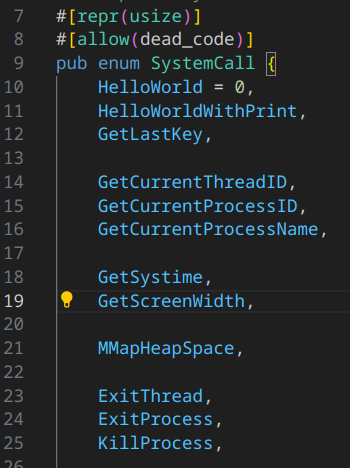
\includegraphics[height=0.8\textheight]{fig/Code Screens/Enum1.png} 
    \end{minipage}
    \hfill
    \begin{minipage}[t]{0.65\textwidth}
        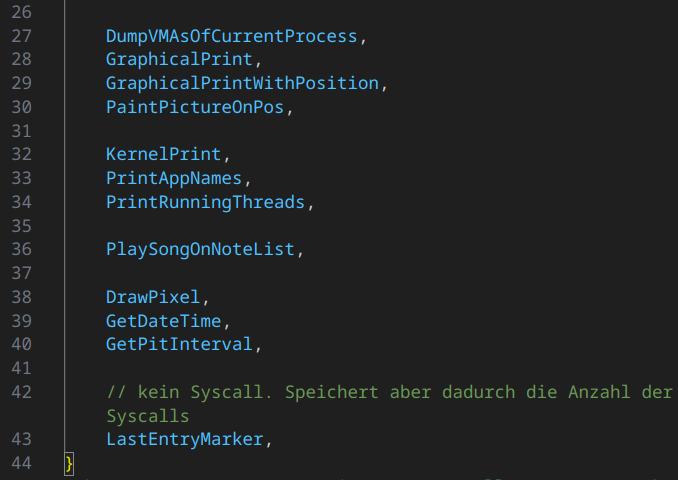
\includegraphics[height=0.8\textheight]{fig/Code Screens/Enum2.png} 
    \end{minipage}
\end{frame}